\documentclass[11pt,a4paper]{article}

\usepackage[utf8]{inputenc}
\usepackage[T1]{fontenc}
\usepackage[spanish,es-nodecimaldot]{babel}
\usepackage{lmodern}
\usepackage{amsmath,amssymb}
\usepackage[margin=2cm]{geometry}
\usepackage{graphicx}
\usepackage{booktabs}
\usepackage{float}
\usepackage{needspace}
\usepackage{listings}
\usepackage{xcolor}
\usepackage[round,authoryear]{natbib}
\usepackage[hidelinks]{hyperref}

\usepackage{tikz}
\usetikzlibrary{arrows.meta,shapes.geometric,backgrounds}
\definecolor{diagramInk}{HTML}{183D2B}
\definecolor{diagramGreen}{HTML}{327A4D}
\definecolor{diagramTeal}{HTML}{236442}
\definecolor{diagramSage}{HTML}{789B4A}
\tikzset{
    diagram/process/.style={
        rectangle, rounded corners=2mm,
        draw=diagramGreen!75!black, fill=diagramGreen!5,
        text=diagramInk, line width=0.7pt,
        align=center, font=\small, inner sep=6pt,
        text width=3.7cm, minimum height=0.95cm
    },
    diagram/output/.style={
        diagram/process, draw=diagramTeal, fill=diagramTeal!7
    },
    diagram/decision/.style={
        diamond, aspect=2.1,
        draw=diagramSage!85!black, fill=diagramSage!12,
        text=diagramInk, line width=0.7pt,
        align=center, font=\small, inner sep=2pt,
        text width=1.85cm, minimum height=1.25cm
    },
    diagram/terminal/.style={
        rectangle, rounded corners=4mm,
        draw=diagramInk, fill=diagramInk, text=white,
        font=\small\bfseries, minimum width=2.3cm,
        minimum height=0.65cm, inner sep=4pt
    },
    diagram/line/.style={
        draw=diagramInk!80, line width=0.8pt, rounded corners=2mm
    },
    diagram/arrow/.style={
        diagram/line, -{Latex[length=2.4mm,width=1.6mm]}
    },
    diagram/night line/.style={diagram/line, draw=diagramGreen},
    diagram/night arrow/.style={diagram/arrow, draw=diagramGreen},
    diagram/repeat arrow/.style={
        diagram/arrow, draw=diagramTeal, dashed
    },
    diagram/edge label/.style={
        font=\scriptsize, text=diagramInk, fill=white, inner sep=2pt
    },
    diagram/night region/.style={
        draw=diagramGreen!25, fill=diagramGreen!2,
        rounded corners=3mm, line width=0.6pt
    },
    diagram/group label/.style={
        font=\scriptsize\bfseries, text=diagramGreen, inner sep=0pt
    },
    diagram/histogram card/.style={
        rectangle, rounded corners=2mm,
        draw=diagramGreen!35, fill=white, line width=0.7pt,
        minimum width=5.2cm, minimum height=6.15cm
    },
    diagram/card title/.style={
        font=\small\bfseries, text=diagramGreen
    },
    diagram/card note/.style={
        font=\small, text=diagramInk
    }
}


\lstset{
    language=Python,
    basicstyle=\ttfamily\footnotesize,
    keywordstyle=\color{blue!60!black},
    stringstyle=\color{green!35!black},
    breaklines=true,
    columns=fullflexible,
    keepspaces=true,
    showstringspaces=false,
    frame=single
}
\setlength{\emergencystretch}{2em}
\renewcommand{\arraystretch}{1.15}
\newcommand{\E}{\mathbb{E}}
\newcommand{\Var}{\operatorname{Var}}

\title{Astroestadística --- Tarea 1\\[0.4em]
\large Detección de microlentes gravitacionales}
\author{Daniel Soto Villada\\
Instituto de Física\\
Universidad de Antioquia}
\date{Semestre 2026-2}

\begin{document}
\maketitle

\section*{Enunciado general}

Una red de telescopios automáticos está diseñada para detectar eventos de microlente gravitacional, que ocurren de forma rara y aleatoria en ciertas regiones del cielo. Suponga que cada noche se monitoriza una región del cielo donde la probabilidad de observar un evento de microlente es de $p = 0.002$, y se realizan observaciones independientes cada noche.

\section*{Solución}

\Needspace{10\baselineskip}
\subsection*{Inciso a}

\begin{quote}
\textbf{a.} Simule el proceso de observación noche a noche hasta obtener un total de $3$ detecciones. Repita el experimento $N = 100, 1000, 10000$ veces y construya una distribución empírica del número de noches $X$ necesarias para las $3$ detecciones.
\end{quote}

\paragraph{Solución.}

Se simula el proceso de observación noche a noche con $p=0.002$ y $r=3$. Para cada experimento se inicializan los contadores de noches y detecciones en cero. En cada noche se genera un número aleatorio mediante \texttt{np.random.random()}; si es menor que $p$, se suma una detección. El proceso continúa hasta obtener las tres detecciones, y se guarda el número total de noches en \texttt{resultados\_X}.

Este procedimiento se repite $N=100$, $1000$ y $10000$ veces. Para cada valor de $N$, los resultados se convierten en un arreglo \texttt{X}, a partir del cual se calculan la media y la varianza y se construye el histograma. Los histogramas obtenidos se presentan en el inciso d y el código se conserva en el apéndice.

\begin{figure}[H]
    \centering
    \begin{tikzpicture}
    \node[diagram/terminal] (inicio) at (0,0) {Inicio};
    \node[diagram/process, text width=4.5cm] (parametros) at (0,-1.35)
        {$p=0.002$, $r=3$\\
         $N\in\{100,1000,10000\}$\\
         $j\gets1$; lista vacía};
    \node[diagram/process] (reiniciar) at (0,-2.9)
        {\texttt{noches} $\gets0$\\\texttt{detecciones} $\gets0$};
    \node[diagram/decision, text width=2.05cm] (faltan) at (0,-5.1)
        {¿Detecciones\\$<r$?};
    \node[diagram/process] (noche) at (0,-6.95)
        {\texttt{noches} $\gets$ \texttt{noches} $+1$\\
         Generar $U\sim\operatorname{Unif}[0,1)$};
    \node[diagram/decision, text width=1.55cm] (detectar) at (0,-8.85)
        {\mbox{¿$U<p$?}};
    \node[diagram/process, text width=2.6cm] (deteccion) at (3.7,-8.85)
        {Incrementar en 1\\\texttt{detecciones}};
    \coordinate (unir) at (0,-10.45);
    \node[diagram/output, text width=3.6cm] (guardar) at (7.5,-5.1)
        {Guardar $X_j=\texttt{noches}$\\en \texttt{resultados\_X}};
    \node[diagram/decision, text width=1.55cm] (repetir) at (7.5,-7.05)
        {\mbox{¿$j<N$?}};
    \node[diagram/process, text width=2.8cm] (siguiente) at (7.5,-2.9)
        {Nueva repetición\\$j\gets j+1$};
    \node[diagram/output, text width=3.6cm] (estadisticas) at (7.5,-9.75)
        {Media y varianza\\Histograma de $X$\\Comparación con la teoría};
    \node[diagram/terminal] (fin) at (7.5,-11.35) {Fin};

    \begin{scope}[on background layer]
        \filldraw[diagram/night region]
            (-3.6,-3.7) rectangle (5.3,-10.85);
    \end{scope}
    \node[diagram/group label, anchor=north west] at (-3.4,-3.85)
        {CICLO DE NOCHES};

    \draw[diagram/arrow] (inicio) -- (parametros);
    \draw[diagram/arrow] (parametros) -- (reiniciar);
    \draw[diagram/arrow] (reiniciar) -- (faltan);
    \draw[diagram/night arrow] (faltan) --
        node[diagram/edge label, right] {Sí} (noche);
    \draw[diagram/night arrow] (noche) -- (detectar);
    \draw[diagram/night arrow] (detectar) --
        node[diagram/edge label, above] {Sí} (deteccion);
    \draw[diagram/night line] (detectar.south) --
        node[diagram/edge label, right] {No} (unir);
    \draw[diagram/night line] (deteccion.south) |- (unir);
    \fill[diagramGreen] (unir) circle (1.6pt);
    \draw[diagram/night arrow] (unir) -- (-3.05,-10.45)
        -- node[diagram/edge label, sloped, above] {Otra noche}
        (-3.05,-5.1) -- (faltan.west);
    \draw[diagram/arrow] (faltan.east) --
        node[diagram/edge label, above] {No: $r=3$ alcanzado} (guardar.west);
    \draw[diagram/arrow] (guardar) -- (repetir);
    \draw[diagram/repeat arrow] (repetir.east) --
        node[diagram/edge label, above] {Sí} (10.2,-7.05)
        -- node[diagram/edge label, sloped, below] {Otra simulación}
        (10.2,-2.9) -- (siguiente.east);
    \draw[diagram/repeat arrow] (siguiente.west) -- (reiniciar.east);
    \draw[diagram/arrow] (repetir) --
        node[diagram/edge label, right] {No: se completó $N$}
        (estadisticas);
    \draw[diagram/arrow] (estadisticas) -- (fin);
\end{tikzpicture}
    \caption{Simulación noche a noche hasta alcanzar tres detecciones. El ciclo verde recorre las noches de un experimento; las flechas verdes discontinuas repiten el experimento hasta completar $N$ simulaciones.}
    \label{fig:flujo-tres-detecciones}
\end{figure}

\Needspace{10\baselineskip}
\subsection*{Inciso b}

\begin{quote}
\textbf{b.} Para cada valor de $N$, calcule la media y la varianza empíricas de $X$. Analice cómo cambian estos valores al aumentar el número de simulaciones. ¿Qué tipo de distribución debería seguir $X$? Justifique.
\end{quote}

\paragraph{Solución.}

Para cada valor de $N$, el cuaderno calcula la media con \texttt{np.mean(X)} y la varianza con \texttt{np.var(X)}. Los resultados guardados son:

\begin{table}[H]
    \centering
    \caption{Media, varianza y tiempo de ejecución de la simulación de $X$.}
    \label{tab:simulacion-x}
    \begin{tabular}{rrrr}
        \toprule
        $N$ & Media (noches) & Varianza (noches$^2$) & Tiempo (s)\\
        \midrule
        100   & 1438.42 & 558325.66 & 0.132\\
        1000  & 1483.51 & 758443.61 & 1.069\\
        10000 & 1482.45 & 717427.70 & 10.960\\
        \bottomrule
    \end{tabular}
\end{table}

A medida que aumenta $N$, la media y la varianza empírica, convergen a sus valores poblacionales.
El tiempo de ejecución escala linealmente. $\mathcal{O}(N)$

Con $r$ y $p$ fijos, esta dependencia lineal se observa también en los tiempos de ejecución del cuaderno. La convergencia de los momentos empíricos no exige que el error disminuya en cada muestra: las diferencias entre $N=1000$ y $N=10000$ corresponden a fluctuaciones de la simulación.

$X$ debería seguir una \textbf{Distribución Binomial Negativa}, porque se cuenta el número de noches necesarias para alcanzar un número fijo de detecciones, con observaciones independientes y probabilidad de éxito constante \citep[sec.~3.5, pp.~118--119]{devore2008}.

\Needspace{10\baselineskip}
\subsection*{Inciso c}

\begin{quote}
\textbf{c.} Con base en las características del experimento, ¿Qué distribución de probabilidad conocida puede modelar la variable $X$?. ¿Cuáles son sus parámetros y por qué es apropiada?
\end{quote}

\paragraph{Solución.}
$X$ sigue una Distribución Binomial Negativa

El experimento satisface exactamente las condiciones de definición de esta distribución

\begin{itemize}
    \item Se realizan ensayos de Bernoulli independientes e idénticamente distribuidos.
    \item La probabilidad de éxito se mantiene constante en cada ensayo ($p=0.002$).
    \item La variable aleatoria $X$ mide el número total de ensayos necesarios para alcanzar un número fijo y predefinido de éxitos ($r=3$) a diferencia de la Binomial, que fija los ensayos y cuenta los éxitos.
\end{itemize}

\textbf{Parámetros de los que depende}

\begin{itemize}
    \item $r=3$: El número fijo de éxitos (detecciones) que se desea alcanzar.
    \item $p=0.002$: La probabilidad constante de éxito en cada ensayo independiente (cada noche).
\end{itemize}

La función de masa de probabilidad para el número total de ensayos $X$ hasta obtener el r-ésimo éxito es:

\[
P(X=x) = \binom{x-1}{r-1}p^r(1-p)^{x-r}
\]

El soporte de esta variable es $x=r,r+1,r+2,\ldots$. Estas condiciones y la función de masa corresponden al modelo binomial negativo \citep[sec.~3.5, p.~119]{devore2008}.

\paragraph{Precisión sobre la definición.}
Devore cuenta el número de fallos anteriores al éxito número $r$. En esta tarea, $X$ cuenta el total de noches, es decir, fallos más $r$ éxitos. El libro reconoce ambas convenciones \citep[p.~119]{devore2008}.

\Needspace{10\baselineskip}
\subsection*{Inciso d}

\begin{quote}
\textbf{d.} Construya histogramas de los resultados de cada experimento y compare con la distribución teórica adecuada. ¿Qué tanto concuerdan ambas distribuciones? ¿Qué pasa cuando $N$ se hace más grande?
\end{quote}

\paragraph{Solución.}

En el cuaderno se construyen histogramas normalizados con \texttt{density=True}, usando intervalos de $100$ noches. Sobre cada histograma se superpone la función de masa teórica de la Binomial Negativa,
\[
    P(X=x)=\binom{x-1}{r-1}p^r(1-p)^{x-r},
\]
calculada mediante la función \texttt{pmf\_teorica}.

\begin{figure}[H]
    \centering
    \begin{tikzpicture}
    \node[diagram/histogram card] (pequena) at (0,0) {};
    \node[diagram/histogram card] (intermedia) at (5.5,0) {};
    \node[diagram/histogram card] (grande) at (11,0) {};

    \node[diagram/card title] at (0,2.75) {MUESTRA PEQUEÑA};
    \node[diagram/card title] at (5.5,2.75) {MUESTRA INTERMEDIA};
    \node[diagram/card title] at (11,2.75) {MUESTRA GRANDE};

    \node[inner sep=0pt] at (0,0.05)
        {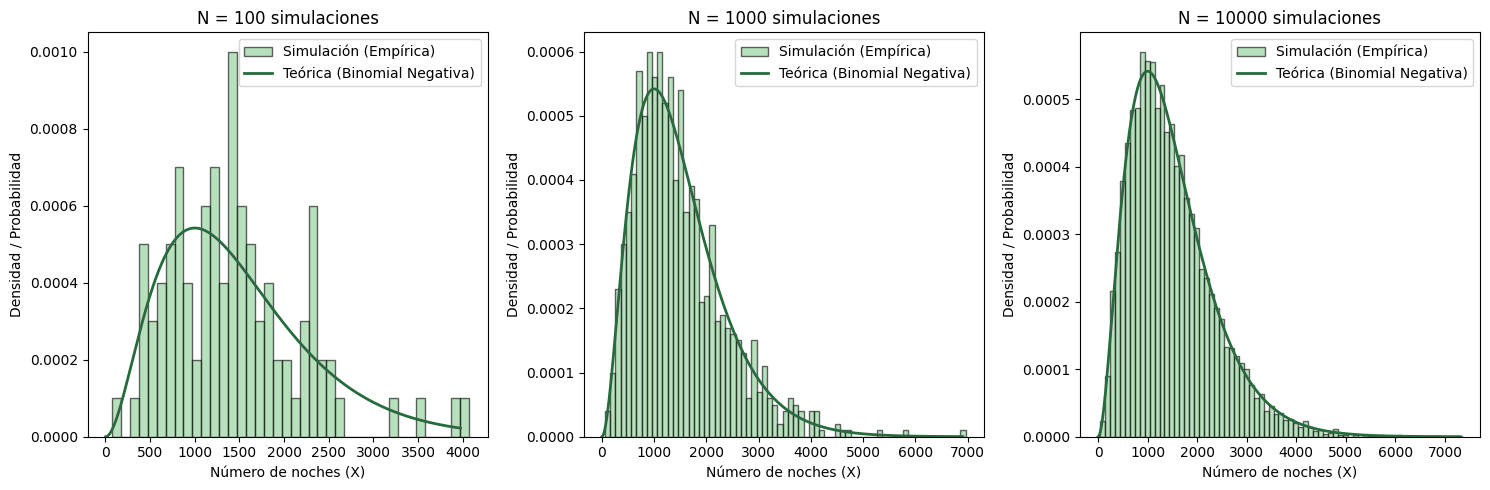
\includegraphics[width=4.9cm,trim={0bp 0bp 712.8bp 0bp},clip]
            {figuras/histogramas.png}};
    \node[inner sep=0pt] at (5.5,0.05)
        {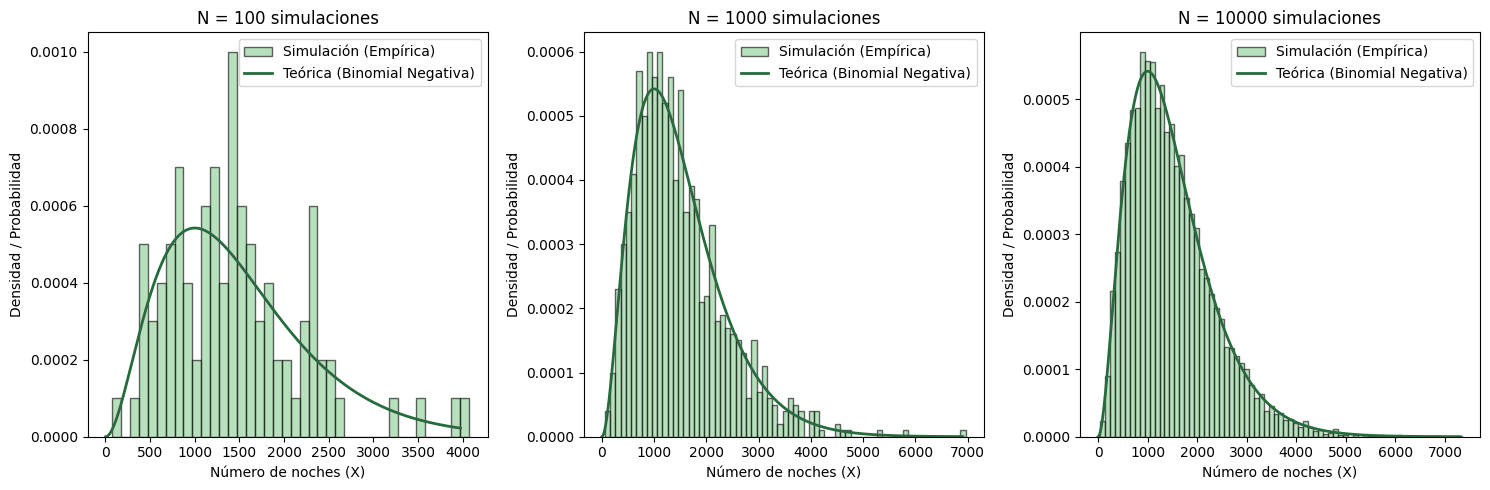
\includegraphics[width=4.9cm,trim={360bp 0bp 360bp 0bp},clip]
            {figuras/histogramas.png}};
    \node[inner sep=0pt] at (11,0.05)
        {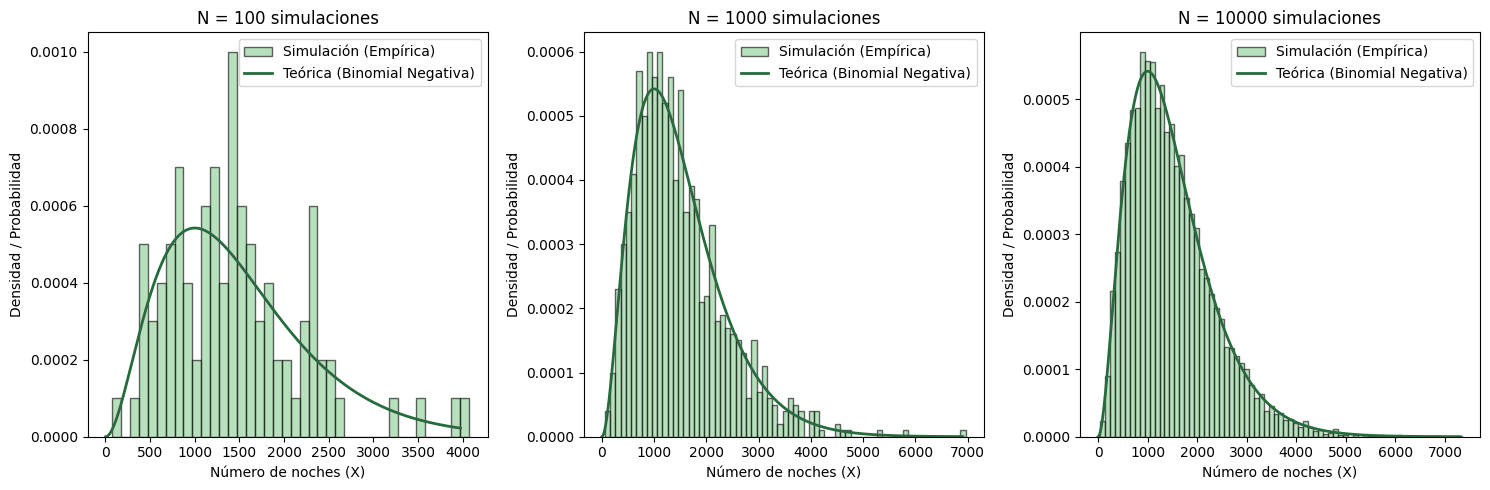
\includegraphics[width=4.9cm,trim={712.8bp 0bp 0bp 0bp},clip]
            {figuras/histogramas.png}};

    \node[diagram/card note] at (0,-2.8) {Alta variabilidad};
    \node[diagram/card note] at (5.5,-2.8) {Menores fluctuaciones};
    \node[diagram/card note] at (11,-2.8) {Mayor acuerdo visual};

    \draw[diagram/arrow, draw=diagramTeal, line width=1.2pt]
        (0,-3.65) -- (11,-3.65);
    \node[diagram/edge label, font=\small\bfseries,
          text=diagramTeal] at (5.5,-3.65)
        {Aumento del número de simulaciones};
    \node[align=center, font=\small, text=diagramInk,
          text width=15cm] at (5.5,-4.4)
        {La distribución empírica se aproxima a la teórica\\
         y el ruido muestral se reduce.};
\end{tikzpicture}
    \caption{Comparación de los histogramas del cuaderno con una paleta verde para $N=100$, $1000$ y $10000$. Las barras representan la simulación y la línea verde oscura, la función de masa teórica de la Binomial Negativa. La flecha destaca el aumento del número de simulaciones y la reducción del ruido muestral.}
    \label{fig:histogramas}
\end{figure}

Con $N=100$, el histograma presenta mayor variabilidad y diferencias visibles respecto a la curva teórica. Al aumentar a $N=1000$ y $N=10000$, las fluctuaciones se reducen y la forma empírica se aproxima mejor a la distribución teórica. Esto concuerda con la observación del cuaderno: a medida que aumenta $N$, los resultados empíricos se aproximan a sus valores poblacionales.



\Needspace{10\baselineskip}
\subsection*{Inciso e}

\begin{quote}
\textbf{e.} Calcule la esperanza y varianza teóricas, y compárelas con los resultados de la simulación.
\end{quote}

\paragraph{Solución.}
Para $X \sim \mathrm{BN}(r, p)$ con $x \in \{r, r+1, r+2, \dots\}$, el valor esperado es:
\[
E[X] = \frac{r}{p}
\]
y la varianza es:
\[
Var(X) = \frac{r(1-p)}{p^2}
\]

Estos momentos se obtienen al usar la convención de total de ensayos. En la convención de fallos de Devore, la esperanza es $r(1-p)/p$; al sumar los $r$ éxitos se obtiene $r/p$, mientras que la varianza no cambia \citep[p.~120]{devore2008}.

Sustituyendo los parámetros del problema,
\[
    E[X]=\frac{3}{0.002}=1500\ \text{noches},
\]
\[
    \Var(X)=\frac{3(1-0.002)}{(0.002)^2}
    =748500\ \text{noches}^2.
\]
Son los mismos valores impresos en el cuaderno: $E[X]=1500.00$ y $\Var(X)=748500.00$.

Al compararlos con la tabla~\ref{tab:simulacion-x}, las medias para $N=1000$ y $N=10000$ son cercanas a $1500$, y las varianzas se aproximan más a $748500$ que la obtenida con $N=100$. La aproximación no es monótona, pero los resultados son consistentes con la convergencia señalada en la solución original. La varianza reportada conserva la definición usada por \texttt{np.var(X)}, con divisor $N$.

\Needspace{10\baselineskip}
\subsection*{Inciso f}

\begin{quote}
\textbf{f.} Ahora, suponga que se realizan observaciones durante exactamente $100$ noches. Simule el experimento y determine el número de detecciones obtenidas en dicho tiempo ($Y$). Repita este procedimiento un número suficientemente grande de veces para estimar, mediante simulación, la probabilidad de realizar al menos una detección
\end{quote}

\paragraph{Solución.}

Se fija el número de noches en $n_{\text{noches}}=100$ y se repite el experimento para $N=100$, $1000$ y $10000$. En cada repetición se cuentan las detecciones obtenidas durante las cien noches y se asigna ese número a $Y$. Si $Y\geq1$, se incrementa el contador \texttt{exitos}. La estimación de la probabilidad es la frecuencia relativa
\[
    \texttt{prob\_empirica}
    =\frac{\text{experimentos con al menos una detección}}{N}.
\]

\begin{table}[H]
    \centering
    \caption{Estimaciones guardadas en el cuaderno para cien noches de observación.}
    \label{tab:simulacion-y}
    \begin{tabular}{rrr}
        \toprule
        $N$ & $P(Y\geq1)$ empírica & Tiempo (s)\\
        \midrule
        100   & 0.14000 & 0.009\\
        1000  & 0.19100 & 0.074\\
        10000 & 0.18320 & 0.608\\
        \bottomrule
    \end{tabular}
\end{table}

Tomando el mayor número de repeticiones, la estimación obtenida es $P(Y\geq1)\approx0.18320$.

\begin{figure}[H]
    \centering
    \begin{tikzpicture}
    \node[diagram/terminal] (inicio) at (0,0) {Inicio};
    \node[diagram/process, text width=4.5cm] (parametros) at (0,-1.4)
        {$p=0.002$, $n=100$, fijar $N$\\
         $j\gets1$; \texttt{exitos} $\gets0$};
    \node[diagram/process] (reiniciar) at (0,-3)
        {\texttt{noche} $\gets0$\\\texttt{detecciones} $\gets0$};
    \node[diagram/decision] (faltan) at (0,-5.3)
        {¿\texttt{noche}\\$<100$?};
    \node[diagram/process] (noche) at (0,-7.2)
        {\texttt{noche} $\gets$ \texttt{noche} $+1$\\
         Generar $U\sim\operatorname{Unif}[0,1)$};
    \node[diagram/decision, text width=1.55cm] (detectar) at (0,-9.05)
        {\mbox{¿$U<p$?}};
    \node[diagram/process, text width=2.6cm] (deteccion) at (3.7,-9.05)
        {Incrementar en 1\\\texttt{detecciones}};
    \coordinate (unirnoches) at (0,-10.55);
    \node[diagram/output, text width=3.5cm] (guardar) at (7.5,-5.3)
        {Periodo de 100 noches completo\\$Y\gets\texttt{detecciones}$};
    \node[diagram/decision, text width=1.7cm] (almenosuna) at (7.5,-7.25)
        {\mbox{¿$Y\geq1$?}};
    \node[diagram/process, text width=3.5cm] (exito) at (7.5,-9.05)
        {\texttt{exitos} $\gets$ \texttt{exitos} $+1$};
    \coordinate (unirexperimentos) at (7.5,-10.55);
    \node[diagram/decision, text width=1.55cm] (repetir) at (7.5,-11.95)
        {\mbox{¿$j<N$?}};
    \node[diagram/process, text width=2.8cm] (siguiente) at (7.5,-3)
        {Nueva repetición\\$j\gets j+1$};
    \node[diagram/output, text width=3.6cm] (estimar) at (7.5,-13.9)
        {Estimar $P(Y\geq1)$\\
         $\widehat P=\texttt{exitos}/N$};
    \node[diagram/terminal] (fin) at (7.5,-15.4) {Fin};

    \begin{scope}[on background layer]
        \filldraw[diagram/night region]
            (-3.6,-3.85) rectangle (5.3,-10.95);
    \end{scope}
    \node[diagram/group label, anchor=north west, align=left] at (-3.4,-4)
        {CICLO DE\\100 NOCHES};

    \draw[diagram/arrow] (inicio) -- (parametros);
    \draw[diagram/arrow] (parametros) -- (reiniciar);
    \draw[diagram/arrow] (reiniciar) -- (faltan);
    \draw[diagram/night arrow] (faltan) --
        node[diagram/edge label, right] {Sí} (noche);
    \draw[diagram/night arrow] (noche) -- (detectar);
    \draw[diagram/night arrow] (detectar) --
        node[diagram/edge label, above] {Sí} (deteccion);
    \draw[diagram/night line] (detectar.south) --
        node[diagram/edge label, right] {No} (unirnoches);
    \draw[diagram/night line] (deteccion.south) |- (unirnoches);
    \fill[diagramGreen] (unirnoches) circle (1.6pt);
    \draw[diagram/night arrow] (unirnoches) -- (-3.05,-10.55)
        -- node[diagram/edge label, sloped, above] {Siguiente noche}
        (-3.05,-5.3) -- (faltan.west);
    \draw[diagram/arrow] (faltan.east) --
        node[diagram/edge label, above] {No: se completó $n=100$} (guardar.west);
    \draw[diagram/arrow] (guardar) -- (almenosuna);
    \draw[diagram/arrow] (almenosuna) --
        node[diagram/edge label, right] {Sí} (exito);
    \draw[diagram/line] (almenosuna.east) --
        node[diagram/edge label, above] {No} (10,-7.25)
        -- (10,-10.55) -- (unirexperimentos);
    \draw[diagram/line] (exito) -- (unirexperimentos);
    \fill[diagramInk] (unirexperimentos) circle (1.6pt);
    \draw[diagram/arrow] (unirexperimentos) -- (repetir);
    \draw[diagram/repeat arrow] (repetir.east) --
        node[diagram/edge label, above] {Sí} (11.2,-11.95)
        -- node[diagram/edge label, sloped, below] {Otra simulación}
        (11.2,-3) -- (siguiente.east);
    \draw[diagram/repeat arrow] (siguiente.west) -- (reiniciar.east);
    \draw[diagram/arrow] (repetir) --
        node[diagram/edge label, right] {No: se completó $N$}
        (estimar);
    \draw[diagram/arrow] (estimar) -- (fin);
\end{tikzpicture}
    \caption{Simulación de detecciones durante exactamente cien noches. El ciclo verde mantiene fijo el periodo de observación; después se comprueba si $Y\geq1$ y se estima su probabilidad mediante la frecuencia relativa de $N$ experimentos.}
    \label{fig:flujo-cien-noches}
\end{figure}

\Needspace{10\baselineskip}
\subsection*{Inciso g}

\begin{quote}
\textbf{g.} Identifique una distribución de probabilidad apropiada para modelar $Y$, Especifique sus parámetros y calcule $P(Y\geq 1)$. Compare este resultado con la estimación obtenida en la simulación.
\end{quote}

\paragraph{Solución.}
La variable aleatoria $Y$, que representa el número de detecciones (éxitos) en un número fijo de noches ($n=100$), sigue una Distribución Binomial.

Esto se debe a que el experimento cumple con las cuatro condiciones de un proceso de Bernoulli:

\begin{itemize}
    \item El número de ensayos es fijo ($n=100$).
    \item Cada ensayo tiene solo dos resultados posibles (detección o no detección).
    \item La probabilidad de éxito es constante en cada ensayo($p=0.002$).
    \item Los ensayos son independientes entre sí.
\end{itemize}

Estas son las condiciones del experimento binomial descritas por Devore \citep[sec.~3.4, p.~108]{devore2008}. Sus parámetros son $n=100$ y $p=0.002$.

Para $Y\sim\text{Bin}(n,p)$, la probabilidad de observar exactamente $y$ éxitos está dada por su función de masa de probabilidad (FMP) \citep[pp.~110--111]{devore2008}:
\[
    P(Y=y)=\binom{n}{y}p^y(1-p)^{n-y},
    \quad y\in\{0,1,2,\dots,n\}.
\]

La probabilidad de obtener al menos una detección es el complemento de la probabilidad de obtener cero detecciones:

\[
P(Y \geq 1) = 1 - P(Y = 0)
\]

Usando la función de masa de probabilidad de la Binomial:
\[
P(Y = 0) = \binom{100}{0} (0.002)^0 (1 - 0.002)^{100} = (0.998)^{100}
\]

Por lo tanto:
\[
P(Y \geq 1) = 1 - (0.998)^{100} \approx 1 - 0.81857 = 0.18143
\]

Comparación con la estimación de la simulación

Tomando el resultado de la simulación con el mayor número de repeticiones ($N = 10000$):

\begin{itemize}
    \item \textbf{Probabilidad teórica exacta:} $0.18143$
    \item \textbf{Probabilidad empírica ($N=10000$):} $0.18320$
\end{itemize}

\textbf{Análisis de la comparación:}
La diferencia absoluta entre el valor teórico y la estimación con $N=10000$ es de apenas $|0.18320 - 0.18143| = 0.00177$ (un error relativo de $\approx0.97\%$).

Este resultado es consistente con que, al aumentar el número de simulaciones, la frecuencia relativa converge al valor de probabilidad real, de acuerdo con la Ley de los Grandes Números. La comparación respalda tanto el modelo Binomial elegido como la consistencia del estimador por simulación.

\Needspace{10\baselineskip}
\subsection*{Inciso h}

\begin{quote}
\textbf{h.} Suponga ahora que el número de noches $n$ aumenta mientras que la probabilidad de detección por noche $p$ disminuye, manteniendo constante el producto $np$ ¿Qué distribución puede utilizarse como aproximación para describir el número de eventos observados?
\end{quote}

\paragraph{Solución.}
La distribución que puede utilizarse como aproximación es la \textbf{Distribución de Poisson}.

Cuando el número de ensayos $n$ tiende a infinito ($n \to \infty$) y la probabilidad de éxito $p$ tiende a cero ($p \to 0$), de tal manera que su producto se mantiene constante e igual a $\lambda$ (es decir, $np = \lambda$), la función de masa de probabilidad de la variable aleatoria $Y \sim \text{Bin}(n, p)$ converge a la de una variable de Poisson.

Matemáticamente, el límite de la probabilidad binomial es:
\[
\lim_{\substack{n \to \infty, p \to 0 \\ np = \lambda}} \binom{n}{y} p^y (1-p)^{n-y} = \frac{e^{-\lambda} \lambda^y}{y!}
\]

La distribución de Poisson resultante tiene un único parámetro $\lambda$, que representa el número esperado de eventos (detecciones) en el intervalo de tiempo considerado:
\[
\lambda = np
\]

Como regla práctica de Devore, esta aproximación puede utilizarse cuando $n \geq 50$ y $np \leq 5$ (``eventos raros en muchos ensayos'') \citep[p.~122]{devore2008}.

En nuestro contexto astroestadístico, los eventos de microlente gravitacional son extremadamente raros ($p = 0.002$), lo que hace de la Poisson un modelo natural para aproximar la Binomial en estos casos.

\Needspace{10\baselineskip}
\subsection*{Inciso i}

\begin{quote}
\textbf{i.} Utilizando dicha aproximación, calcule la probabilidad de observar al menos un evento durante $100$ noches. Compare este resultado con la probabilidad exacta obtenida anteriormente y con la estimación de la simulación.
\end{quote}

\paragraph{Solución.}
Cuando el número de ensayos $n$ es grande y la probabilidad de éxito $p$ es muy pequeña, la distribución Binomial puede aproximarse mediante una \textbf{distribución de Poisson} con parámetro $\lambda = np$.

Para nuestro experimento de $n = 100$ noches y $p = 0.002$:
\[
\lambda = 100 \times 0.002 = 0.2
\]

La probabilidad de observar al menos un evento ($Y \geq 1$) usando la aproximación de Poisson es el complemento de no observar ningún evento ($Y = 0$):
\[
P(Y \geq 1) \approx 1 - P(Y = 0) = 1 - \frac{e^{-\lambda} \lambda^0}{0!} = 1 - e^{-0.2}
\]
\[
P(Y \geq 1) \approx 1 - 0.81873 = \mathbf{0.18127}
\]

La función de masa de Poisson y su relación con la distribución Binomial se presentan en la sección 3.6 de Devore \citep[pp.~121--122]{devore2008}.

\paragraph{Comparación de Resultados.}
A continuación, contrastamos los tres enfoques utilizados a lo largo de la tarea para resolver este mismo problema:

\begin{table}[H]
    \centering
    \caption{Comparación de la aproximación, el cálculo exacto y la simulación.}
    \begin{tabular}{lll}
        \toprule
        Método & Fórmula / Origen & Probabilidad $P(Y\geq1)$\\
        \midrule
        Aproximación (Poisson) & $1-e^{-0.2}$ & 0.18127\\
        Exacta (Binomial) & $1-(1-0.002)^{100}$ & 0.18143\\
        Simulación ($N=10000$) & Frecuencia relativa empírica & $\approx0.18320$\\
        \bottomrule
    \end{tabular}
\end{table}

\paragraph{Análisis y Conclusión.}
\begin{enumerate}
    \item \textbf{Precisión de la Aproximación:} La diferencia absoluta entre el cálculo exacto (Binomial) y la aproximación (Poisson) es de apenas $|0.18127-0.18143|=0.00016$. Este error es muy pequeño, lo que demuestra que la distribución de Poisson es un modelo matemático excelente y computacionalmente más sencillo para describir la ocurrencia de \textbf{eventos raros} (como las microlentes gravitacionales) en intervalos de tiempo fijos. Esto es consistente con la regla práctica de Devore, que sugiere usar Poisson cuando $n\geq50$ y $np\leq5$ \citep[p.~122]{devore2008}.
    \item \textbf{Validación Empírica:} La estimación obtenida por simulación ($\approx0.18320$) presenta una ligera desviación debido al error de muestreo inherente a generar $N=10000$ experimentos aleatorios. Si aumentáramos $N$ a $1000000$, se esperaría una estimación más precisa del valor teórico $0.18143$, de acuerdo con la convergencia de la frecuencia relativa. Esto respalda el modelo discreto exacto y su comparación con la aproximación asintótica, sin garantizar un resultado específico en una ejecución particular.
\end{enumerate}

\bibliographystyle{plainnat}
\bibliography{referencias}

\clearpage
\appendix
\lstset{basicstyle=\ttfamily\scriptsize, aboveskip=0.5em, belowskip=0.5em}
\section{Código de simulación y cálculos}

Los siguientes bloques recogen el núcleo de los procedimientos del cuaderno, omitiendo las instrucciones de medición de tiempo y construcción de la figura. La figura incluida en el informe es la salida original, no una regeneración. El cuaderno no fija una semilla aleatoria; por ello, una nueva ejecución producirá valores empíricos distintos de los aquí reportados.

\subsection{Tiempo de espera hasta tres detecciones}

\begin{lstlisting}
import numpy as np
p = 0.002
r = 3
Ns = [100, 1000, 10000]
for N in Ns:
    resultados_X = []
    for _ in range(N):
        noches, detecciones = 0, 0
        while detecciones < r:
            noches += 1
            if np.random.random() < p:
                detecciones += 1
        resultados_X.append(noches)
    X = np.array(resultados_X)
    print(f"N={N:5d} | Media: {np.mean(X):.2f} | "
          f"Varianza: {np.var(X):.2f}")
print(f"E[X] = {r/p:.2f}")
print(f"Var(X) = {r*(1-p)/p**2:.2f}")
\end{lstlisting}

\subsection{Detecciones en cien noches}

\begin{lstlisting}
n_noches = 100
for N in Ns:
    exitos = 0
    for _ in range(N):
        detecciones = 0
        for noche in range(n_noches):
            if np.random.random() < p:
                detecciones += 1
        Y = detecciones
        if Y >= 1:
            exitos += 1
    prob_empirica = exitos / N
    print(f"N={N:5d} | P(Y >= 1): {prob_empirica:.5f}")
\end{lstlisting}

\subsection{Probabilidades teóricas y errores}

Este bloque distingue el error absoluto del relativo y usa la estimación guardada para $N=10000$ en la comparación numérica.

\begin{lstlisting}
lam = n_noches * p
p_binomial = 1 - (1 - p)**n_noches
p_poisson = 1 - np.exp(-lam)
prob_guardada = 0.18320
error_absoluto = abs(p_binomial - prob_guardada)
error_relativo = error_absoluto / p_binomial
print(f"Binomial: {p_binomial:.5f}")
print(f"Poisson: {p_poisson:.5f}")
print(f"Error absoluto de simulacion: {error_absoluto:.5f}")
print(f"Error relativo de simulacion: {error_relativo:.3%}")
print(f"Diferencia binomial-Poisson: "
      f"{abs(p_binomial - p_poisson):.5f}")
\end{lstlisting}

\end{document}